% ----------------------- %
% MOCI SOFTWARE LATEX DOC %
% ----------------------- %
%
% DO NOT ADD CONTENT HERE
% only add content in indivudual
% .tex docs and include there bere
%
\documentclass{report}
%
% packages go below here
%
\usepackage{amsmath}
% \usepackage[utf8]{inputenc}
% \usepackage[english]{babel}
\usepackage{graphicx}
\usepackage{biblatex}
\usepackage{mathtools}
\usepackage{amssymb}
\usepackage{subfiles}
\usepackage{titling}
\usepackage{amssymb}
\usepackage{algorithm}
\usepackage{pgfplots}
\usepackage{tikz-3dplot}
\usepackage[noend]{algpseudocode}
\usepackage[margin=1.5cm]{geometry}

\usetikzlibrary{calc,arrows.meta,positioning,backgrounds}
\DeclarePairedDelimiter\floor{\lfloor}{\rfloor}

%
% stuff relating to the title
%
\pretitle{%
  \begin{center}
  \LARGE
  
\includegraphics[width=8cm, height=8cm]{MOCI}\\[\bigskipamount]
}
\title{Multiview Onboard Computaional Imager \\
  \large Algorithm Theoretical Basis Document
}
\author{
  Caleb, Adams\\
  \texttt{CalebAshmoreAdams@gmail.com}
  \and
  LastName2, FirstName2\\
  \texttt{first2.last2@xxxxx.com}
  \and
  LastName3, FirstName3\\
  \texttt{first3.last3@xxxxx.com}
}
\posttitle{
  %
\includegraphics[width=8cm]{ssrl}
  \end{center}
}
%
%
\addbibresource{sources.bib}
\graphicspath{ {./img/} }

%
% DOCUMENT STARTS
%

\begin{document}

\maketitle

\tableofcontents
\addcontentsline{toc}{chapter}{section}


\chapter{Introduction}

\section{Feature Detection}

\section{Feature Discription}

\section{Feature Matching}

\section{2 View Reprojection}

\section{N View Reprojection}

\section{Surface Reconstruction}

\chapter{Feature Detection}

\chapter{Feature Extraction}

\chapter{Feature Matching}

\section{Overview}

\section{2 View Matching}

\section{N View Matching}

\chapter{Two View Reprojection}

\section{Overview}
The goal with the 2-view reprojection is to take the pairs of matched points from the SIFT steps and
move them from $\mathbb{R}^{2}$ into $\mathbb{R}^{3}$ so that equations of lines can be generated from the
focal point of the camera into each matched point. Then, we want to find the minimum distance between those
lines and choose the midpoint of that line segment at our reprojected point.

\section{Getting Equations of Lines}

\begin{center}
\tdplotsetmaincoords{-60}{-35}
\begin{tikzpicture}
  [
    tdplot_main_coords,
    >=Stealth,
    my dashed/.style={dashed, thick, ->, shorten >=-15pt, shorten <=-15pt, every node/.append style={font=\footnotesize}},
    my box/.style={thin, gray!70},
    my blue/.style={blue, line cap=round, -{Triangle[width=3*#1]}, line width=#1, shorten >=#1*1.75pt, every node/.append style={fill, circle, inner sep=0pt, minimum size=#1*3.5pt, anchor=center, outer sep=0pt}},
    my label/.append style={midway, font=\scriptsize},
    my vectors/.style={green!50!black, {Stealth[scale=.75]}-{Stealth[scale=.75]}},
    my red/.style={thick, red, line cap=round},
    my grey/.style={gray!70},
    description/.style={draw=gray!70, thick, line cap=round, every node/.style={align=center, font=\scriptsize\sffamily, anchor=north}},
  ]
  \draw [my grey] (0,4,0) -- (0,7,0) (-2,7,0) -- (2,7,0);
  \coordinate (o) at (0,0,0);

  \path [draw=gray!70, text=gray, fill=gray!20, opacity=0.8, text opacity=1] (-1.5,4,1.75) coordinate (a) -- ++(0,0,-3.5) coordinate (b) -- ++(3,0,0) coordinate (c) -- ++(0,0,3.5) coordinate (d) -- cycle node [pos=.95, above, sloped, anchor=south west] {$z=f$} ;

  \draw [my grey] (-2,0,0) -- (2,0,0) (0,0,0) -- (0,4,0) (0,0,0) -- (0,0,2);
  \draw [thick, ->, every node/.style={font=\footnotesize, inner sep=0pt}] (o) node [anchor=north west] {$C$} (o) edge node [pos=1, anchor=north east] {$C_z$} ++(0,1,0) edge node [pos=1, anchor=north] {$C_y$} ++(0,0,1) -- ++(1,0,0) node [anchor=north west] {$C_x$};
  \draw [my box] (o) ++(0,4,-.5) coordinate (p1) -- ++(1,0,0) coordinate (p2) -- ++(0,0,-1.25) coordinate (p3);
  \foreach \i in {0,1,...,4} \draw [my box] (p1) ++(\i*.25,0,0) -- ++(0,0,-.25);
  \foreach \i in {0,1,...,5} \draw [my box] (p2) ++(0,0,-\i*.25) -- ++(-.25,0,0);

  \draw [my box] (p1) ++(0,0,-.25) -- ++(.75,0,0) -- ++(0,0,-1);
  \draw [my dashed, cyan] ($(b)!1/2!(c)$) -- ($(d)!1/2!(a)$) node [below=15pt, anchor=north] {$y - \frac{res}{2}$};
  \draw [my dashed, cyan] ($(b)!1/2!(a)$) -- ($(d)!1/2!(c)$) node [above right=17pt, anchor=north west] {$x - \frac{res}{2}$};

  \draw [my dashed, green!50!black, <->] (a) node [below=15pt, anchor=north] {$x$} -- (b) -- (c) node [above right=17pt, anchor=north west] {$y$};
  \path [green!50!black, every node/.style={font=\scriptsize, inner sep=0pt}] (p2) node [above right, anchor=south west] {$(x',y')$};

  \path (p2) ++(-.125,0,0) coordinate (q2) ++(0,0,-.125) coordinate (r2);
  \draw ($(0,4,0)+($(q2)-(p1)$)$) coordinate (s2) -- (r2) node (d1) {};
  \scoped[on background layer]{\draw ($($1.75*($(s2)-(0,4,0)$)$)+(0,7,0)$) -- ++($1.75*($(r2)-(s2)$)$) node (d2) {};}
  \draw [my red] (o) node[above] {$\vec{v}$} -- (d1.center);

  \scoped[on background layer]{\draw [my red] (d1.center) -- (d2.center);}

\end{tikzpicture}
\end{center}

The goal here is to generate a parametric equation of a line given camera position and orientation coordinates $C$,
the camera focal length $f$, and the position of a coordinate in $\mathbb{R}^{2}$ on the image plane. We wish to
generate vector $v$ that can be used to make the parametric equation.
The 2-view reprojection takes the matched points between 2 images and places them into $\mathbb{R}^{3}$.
To place each set of points into $\mathbb{R}^{3}$ some trigonometry and and matrix transformations need to take place.
The first step to moving a keypoint into $\mathbb{R}^{3}$ is to place it onto a plane in $\mathbb{R}^{2}$.
the coordinates $(x', y')$ in $\mathbb{R}^{2}$ require the size of a pixel $dpix$, the location of the keypoint $(x, y)$,
and the resolution of the image $(xres, yres)$ to yield:

\[
x' = dpix(x - \frac{xres}{2})\hspace{1cm} y' = dpix(y - \frac{yres}{2})
\label{test}
\]

This is repeated for the other matching keypoint. The coordinate $(x', y', z')$ in $\mathbb{R}^{3}$ of
the keypoint $(x', y')$ in $\mathbb{R}^{2}$ is given by three rotation matrices and one translation matrix.
First we treat $(x', y')$ in $\mathbb{R}^{2}$ as a homogenous vector in $\mathbb{R}^{3}$ to yield $(x', y', 1)$.
Given a unit vector representing the camera, in our case the spacecraft’s
camera’s, orientation $(r_x,r_y,r_z)$ we find the angle to rotate in each axis $(\theta_x,\theta_y,\theta_z)$.
in our simple case we find the angle in the $xy$ plane with:

\[
\theta_z = \cos^{-1} \frac{ (\begin{bmatrix}1 & 0 & 0\end{bmatrix} \cdot \begin{bmatrix}r_x & r_y & r_z \end{bmatrix}) }{ \sqrt{ \begin{bmatrix}r_x & r_y & r_z\end{bmatrix} \cdot \begin{bmatrix}r_x & r_y & r_z\end{bmatrix} } }
\]

Future software will generate rotations for all planes in an identical way.
Now, given a rotation in each plane $(\theta_x,\theta_y,\theta_z)$ we calculate the homogeneous
coordinate $(r_x,r_y,r_z, 1)$ in $\mathbb{R}^{4}$ using linear transformations.
The values $(T_x,T_y,T_z)$ represent a translation in $\mathbb{R}^{3}$ and use camera
position coordinates $(C_x,C_y,C_z)$, the camera unit vectors
representing orientation $(u_x,u_y,u_z)$, and focal length $f$:
%=========
\[
\begin{bmatrix}
  1 & 0 & 0 & 0\\
  0 & \cos(\theta_x) & -\sin(\theta_x) & 0\\
  0 & \sin(\theta_x) & \cos(\theta_x) & 0\\
  0 & 0 & 0 & 1
\end{bmatrix}
\begin{bmatrix}
  \cos(\theta_y) & 0 & \sin(\theta_y) & 0\\
  0 & 1 & 0 & 0\\
  -\sin(\theta_y) & 0 & \cos(\theta_y) & 0\\
  0 & 0 & 0 & 1
\end{bmatrix}
\begin{bmatrix}
  \cos(\theta_z) & -\sin(\theta_z) & 0 & 0\\
  0 & \cos(\theta_x) & -\sin(\theta_x) & 0\\
  0 & 0 & 1 & 0\\
  0 & 0 & 0 & 1
\end{bmatrix}
\begin{bmatrix}
  x\\
  y\\
  z\\
  1
\end{bmatrix}
=
\begin{bmatrix}
  x_r\\
  y_r\\
  z_r\\
  1
\end{bmatrix}
\]
%=========
\[
\begin{bmatrix}
  C_x - (x_r + f * u_x)\\
  C_y - (y_r + f * u_y)\\
  C_z - (z_r + f * u_z)\\
  1
\end{bmatrix}
=
\begin{bmatrix}
  T_x\\
  T_y\\
  T_z\\
  1
\end{bmatrix}
\]
%=========
\[
\begin{bmatrix}
  1 & 0 & 0 & T_x\\
  0 & 1 & 0 & T_y\\
  0 & 0 & 1 & T_z\\
  0 & 0 & 0 & 1
\end{bmatrix}
\begin{bmatrix}
  x_r\\
  y_r\\
  z_r\\
  1
\end{bmatrix}
=
\begin{bmatrix}
  x'_r\\
  y'_r\\
  z'_r\\
  1
\end{bmatrix}
\]

The above process should happen for both points that have been matched.
This should result in 2 homogeneous points that we will call $\begin{bmatrix}x_0 & y_0 & z_0 & 1 \end{bmatrix}^T$
and $\begin{bmatrix}x_1 & y_1 & z_1 & 1 \end{bmatrix}^T$. Each point has a corresponding camera vector,
which is already known thanks to the camera coordinates, $\begin{bmatrix}C_{x0} & C_{y0} & C_{z0} & 1 \end{bmatrix}^T$
and $\begin{bmatrix}C_{x1} & C_{y1} & C_{z1} & 1 \end{bmatrix}^T$. From this we can make parametic lines $L_0$ and $L_1$
with the parametic variables $t_0$ and $t_1$:

\[
L_0 =
\begin{bmatrix}
  x_0 - C_{x0}\\
  y_0 - C_{y0}\\
  z_0 - C_{z0}
\end{bmatrix}
\begin{bmatrix}
  t_0\\
  t_0\\
  t_0
\end{bmatrix}
+
\begin{bmatrix}
  C_{x0}\\
  C_{y0}\\
  C_{z0}
\end{bmatrix}
\]

\[
L_1 =
\begin{bmatrix}
  x_1 - C_{x1}\\
  y_1 - C_{y1}\\
  z_1 - C_{z1}
\end{bmatrix}
\begin{bmatrix}
  t_1\\
  t_1\\
  t_1
\end{bmatrix}
+
\begin{bmatrix}
  C_{x1}\\
  C_{y1}\\
  C_{z1}
\end{bmatrix}
\]

% the other alg

The Host functions are simple and will not be addressed here, refer to standard CUDA memory management.
For the Kernel, we must insure that we have a few global variables about the camera data/parameters
availible to the GPU. These variables are the focal length $foc$, the feild of view $fov$, and the
resolution of the imager $res$. This assumes that the cameras are in the $xy$ plane, which can only
be assumed for this special 2-view case. It may be helpful to read the section on file formats, which
is after the main introduction.

\begin{algorithm}
\caption{Device Kernel}\label{Line Generation Device}
\begin{algorithmic}[1]
  %inside alg
  \State Let: $dpix = foc * \tan{\frac{fov/2}{res/2}}$
  \State Let: $i = blockIdx.x * blockDim.x + threadIdx.x$
  \Procedure{GenerateLines(R2points, R3cameras)}{}
    \State $C_0[6] = (R3cameras[0],R3cameras[1],R3cameras[2],R3cameras[3],R3cameras[4],R3cameras[5])$
    \State $C_1[6] = (R3cameras[6],R3cameras[7],R3cameras[8],R3cameras[9],R3cameras[10],R3cameras[11])$
    \State $x_0 = (R2points[i] - res/2.0)$
    \State $y_0 = (-R2points[i+1]) + res/2.0)$
    \State $x_1 = (R2points[i+2] - res/2.0)$
    \State $y_1 = (-R2points[i+3]) + res/2.0)$
    \State $kp_0 = [x_0,y_0,0.0]$
    \State $kp_1 = [x_1,y_1,0.0]$
    \State $\theta_{x0} = \cos^{-1}(\frac{kp0 \cdot \begin{bmatrix}1 & 0 & 0\end{bmatrix}^{T}}{\sqrt{\|kp_0\|}})$
    \State $\theta_{x1} = \cos^{-1}(\frac{kp1 \cdot \begin{bmatrix}1 & 0 & 0\end{bmatrix}^{T}}{\sqrt{\|kp_1\|}})$
    \State $kp_0 = kp_0 \begin{bmatrix}1 & 0 & 0\\ 0 & \cos(\frac{\pi}{2}) & -\sin(\frac{\pi}{2})\\ 0 & \sin(\frac{\pi}{2}) & \cos(\frac{\pi}{2})\\ \end{bmatrix}    \begin{bmatrix}\cos(\theta_{x0} + \frac{\pi}{2}) & -\sin(\theta_{x0} + \frac{\pi}{2}) & 0\\ \sin(\theta_{x0} + \frac{\pi}{2}) & \cos(\theta_{x0} + \frac{\pi}{2}) & 0\\ 0 & 0 & 1\\ \end{bmatrix}$
    \State $kp_1 = kp_1 \begin{bmatrix}1 & 0 & 0\\ 0 & \cos(\frac{\pi}{2}) & -\sin(\frac{\pi}{2})\\ 0 & \sin(\frac{\pi}{2}) & \cos(\frac{\pi}{2})\\ \end{bmatrix}    \begin{bmatrix}\cos(\theta_{x1} + \frac{\pi}{2}) & -\sin(\theta_{x1} + \frac{\pi}{2}) & 0\\ \sin(\theta_{x1} + \frac{\pi}{2}) & \cos(\theta_{x1} + \frac{\pi}{2}) & 0\\ 0 & 0 & 1\\ \end{bmatrix}$
    \State $kp_0[0] = C_0[0] - (kp_0[0] (C_0[3] * foc))$
    \State $kp_0[1] = C_0[1] - (kp_0[1] (C_0[4] * foc))$
    \Comment kp0 now represents the keypoint location in $\mathbb{R}^{3}$
    \State $kp_1[0] = C_1[0] - (kp_1[0] (C_1[3] * foc))$
    \State $kp_1[1] = C_1[1] - (kp_1[1] (C_1[4] * foc))$
    \Comment kp1 now represents the keypoint location in $\mathbb{R}^{3}$
    \State $v_0 = kp_0 - C_0$
    \Comment line $L_0$'s vector
    \State $v_1 = kp_1 - C_1$
    \Comment line $L_1$'s vector
  \EndProcedure
\end{algorithmic}
\end{algorithm}

In the future, only the first $3$ components, the position coordinates, of $C_0$ and $C_1$ are used.
Vectors $v_0$ and $v_1$ are used to parateterizeds lines.

\newpage
\section{Minimum Distance Between Skew Lines}
Now that we have lines $L_0$ and $L_1$, the challenge is to find the points $s_0$ and $s_1$ of
closest approach. First, we must test the assumption that our lines are skew, meaining they
are not parrallel and do not intersect. To start to think of this we take the forms of $L_0$ and $L_1$
and simplify them by thinking of them as parametic vectors where $C_0$ and $C_1$, represent the camera
position vectors and $v_0$ and $v_1$ represent the vector was previously calculated from the subtraction
of match coordinates with the camera vector. We make the simple equations:

\[
L_0 = v_0 t_0 + C_0 \hspace{1cm} L_1 = v_1 t_1 + C_1
\]

To make sure that the lines are not parallel, which is unlikely, we must verify that their cross product
is not zero. if $v_0 \times v_1 = 0$ then we have a degenerate case with infinitely many solutions. As long
as we know this is not the case we can proceed. We know that the cross product of the two vectors
$c = v_0 \times v_1$ is perpendicular to the lines $L_0$ and $L_1$. We know that the plane $P$, formed by the
translation of $L1$ along $c$, contains $C_1$. We also know
that the point $C_1$ is perpendicular to the vector $n_0 = v_1 \times (v_0 \times v_1)$. Thus, the intersection
of $L_0$ with $P$ is also the point, $s_0$, that is nearest to $L_1$, given by the equation:

\[
s_0 = C_0 + \frac{(C_1 - C_0) \cdot n_0}{v_0 \cdot n_0} \cdot v_0
\]

This also holds for the second line $L_1$, the point $s_1$, and vector $n_1 = v_0 \times (v_1 \times v_0)$.
with the equation:

\[
s_1 = C_1 + \frac{(C_0 - C_1) \cdot n_1}{v_1 \cdot n_1} \cdot v_1
\]

Now, given to points that represent the closest points of approach, we simply find the midpoint $m$:

\[
m = \begin{bmatrix}
  (s_0[x] + s_1[x])/2\\
  (s_0[y] + s_1[y])/2\\
  (s_0[z] + s_1[z])/2
\end{bmatrix}
\]

\section{Least Square Approximation for Two Lines}

\chapter{N/Multiview Reprojection}

\section{Overview}
At this stage we are exclusivley in $\mathbb{R}^{3}$.
For the purpose of our software, we expect points in the form $P = (p_x, p_y, p_z)$
and their corresponding orientation as a unit vector $\hat{U} = (\hat{u}_x, \hat{u}_y, \hat{u}_z)$,
we expect these together in a tuple $ ((p_x, p_y, p_z), (\hat{u}_x, \hat{u}_y, \hat{u}_z))_n $.
This tuple comes with several ($n$ many) tuples which all uniquely correspond with a matched set.
So we have a $\mathbb{R}^{3}$ match set $M = \{ (P, \hat{U})_0, (P, \hat{U})_1, ... , (P, \hat{U})_n \}$
where $n$ is the numnber of tuple pairs and has a one-to-one correspondence with
the number of views in which the $\mathbb{R}^{2}$ match was found.
We all also get a set of $\mathbb{R}^{3}$ matches,
$M_i$,
resulting in a set which has a one-to-one correspondence with the total number
of points we should have after reprojection.

\begin{center}
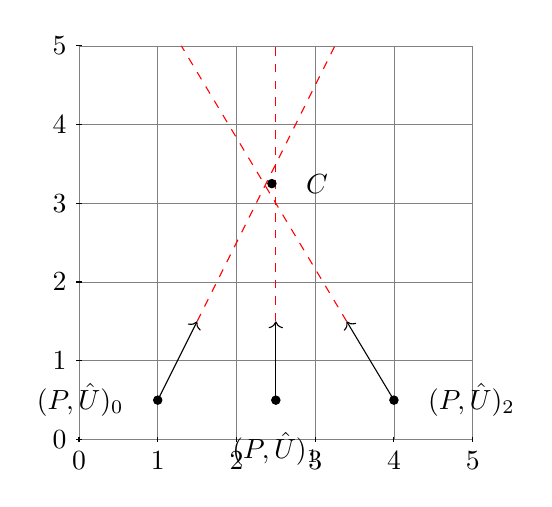
\begin{tikzpicture}

% the grid and stuff
\draw[step=1cm,gray,very thin] (0,0) grid (5,5);
\foreach \x in {0,1,2,3,4,5}
   \draw (\x cm,1pt) -- (\x cm,-1pt) node[anchor=north] {$\x$};
\foreach \y in {0,1,2,3,4,5}
    \draw (1pt,\y cm) -- (-1pt,\y cm) node[anchor=east] {$\y$};

% the arrows
\draw[->](1,0.5) -- (1.5,1.5);
\draw[->](2.5,0.5) -- (2.5,1.5);
\draw[->](4,0.5) -- (3.4,1.5);

% dotted lines
\draw[red,thin,dashed] (1.5,1.5) -- (3.25,5.0);
\draw[red,thin,dashed] (2.5,1.5) -- (2.5,5.0);
\draw[red,thin,dashed] (3.4,1.5) -- (1.3,5.0);

% points
\filldraw (1,0.5) circle[radius=1.5pt];
\node[left=8pt of {(1,0.5)}, outer sep=1pt] {$(P,\hat{U})_0$};
\filldraw (2.5,0.5) circle[radius=1.5pt];
\node[below=8pt of {(2.5,0.5)}] {$(P,\hat{U})_1$};
\filldraw (4,0.5) circle[radius=1.5pt];
\node[right=8pt of {(4,0.5)}, outer sep=1pt] {$(P,\hat{U})_2$};
\filldraw (2.45,3.25) circle[radius=1.5pt];
\node[right=8pt of {(2.45,3.25)}, outer sep=1pt] {$C$};

% labels

\end{tikzpicture}
\end{center}

I know I said we're in $\mathbb{R}^{3}$ (and we are), just imagine that the diagram
above illustrates the values within a particular Z plane. Note that the diagram
could be similar if any arbitary plane is chosen.\\
\\
In the above diagram, assume that point $C$ is the correct real world point and
has no orientation. We're trying to make a best guess at was $C$ is given our
imperfect information.

\section{3 by 3 Inversion Method}
Caleb (me the person writing this) made up the name to this method, so don't
search it because you probably won't find anything about it. \\
\\
First, remember the identity:
\[
(m \times n) \cdot (m \times n) = || m ||^2  || n ||^2 - (m \cdot n)^2
\]
Then note, we have the distance function, measuring how much a given
$((p_x, p_y, p_z), (\hat{u}_x, \hat{u}_y, \hat{u}_z))_n$ tuple (which represents
a line) misses the real world targe point $C$. Not this function is calculated
for each tuple.
\[
D_n = \frac{||(C - P_n) \times \hat{U}_n || }{ || \hat{U}_n ||}
\]
We will want to use the square of the distance (as is common in many optimization
problems) to insure convex optimization and positive distance values. We also use
the identity mentioned above to get our primary distance equation. Then, taking
the first derivative of the distance function will, to find a $0$ solution, will
give us a local minimum value.
\begin{align*}
    D_n &= \frac{||(C - P_n) \times \hat{U}_n || }{ || \hat{U}_n ||} \\
    D_n^2 &= \Big( \frac{||(C - P_n) \times \hat{U}_n || }{ || \hat{U}_n ||} \Big)^2 \\
    D_n^2 &= \frac{||(C - P_n) \times \hat{U}_n ||^2  }{ || \hat{U}_n ||^2 }\\
    D_n^2 &= \frac{ || C - P_n ||^2   || \hat{U}_n ||^2 - ||(C - P_n) \cdot \hat{U}_n ||^2 }{ || \hat{U}_n ||^2 }\\
    D_n^2 &= || C - P_n ||^2  - \frac{ ||(C - P_n) \cdot \hat{U}_n ||^2 }{|| \hat{U}_n ||^2} \\
    \frac{d D_n^2}{d C} &= 2 (C - P_n) - 2 \hat{U}_n  \frac{ (C - P_n) \cdot \hat{U}_n }{ || \hat{U}_n ||^2 }
\end{align*}
So, we need to find a zero for the following (note that we are dealing with a
vector in $\mathbb{R}^{3}$, so $0 = [0 , 0, 0]^T$). the value $m$ is the total number
of $\mathbb{R}^{3}$ match points:

\begin{align*}
  0 &= \sum_{n=0}^m C - P_n - \hat{U}_n \frac{ (C - P_n) \cdot \hat{U}_n }{ || \hat{U}_n ||^2 }\\
  0 &= \sum_{n=0}^m C - P_n - \frac{ \hat{U}_n ( C \cdot \hat{U}_n ) }{ || \hat{U}_n ||^2 } + \frac{ \hat{U}_n ( P_n \cdot \hat{U}_n ) }{ || \hat{U}_n ||^2 } \\
  0 &= \sum_{n=0}^m C - P_n - \frac{ \hat{U}_n \hat{U}_n^T C }{ || \hat{U}_n ||^2 } + \frac{ \hat{U}_n \hat{U}_n^T P_n }{ || \hat{U}_n ||^2 }\\
  0 &= \sum_{n=0}^m \Big( I -  \frac{ \hat{U}_n \hat{U}_n^T }{ || \hat{U}_n ||^2 }  \Big) C - \Big( P_n - \frac{ \hat{U}_n \hat{U}_n^T P_n }{ || \hat{U}_n ||^2 } \Big)
\end{align*}

Notice this is of the form $Ax = b$ because we now have $0 = Ax - b$. The next
thing to note is we can remove the summations and get a system that results in
taking an inverse of a 3 by 3 matrix.\\
\\
Notice the possible expansion:
\begin{align*}
  0 &= \sum_{n=0}^m \Big( I -  \frac{ \hat{U}_n \hat{U}_n^T }{ || \hat{U}_n ||^2 }  \Big) C - \Big( P_n - \frac{ \hat{U}_n \hat{U}_n^T P_n }{ || \hat{U}_n ||^2 } \Big)\\
  0 &= \Bigg( \Big( I -  \frac{ \hat{U}_0 \hat{U}_0^T }{ || \hat{U}_0 ||^2 }  \Big) + \Big( I -  \frac{ \hat{U}_1 \hat{U}_1^T }{ || \hat{U}_1 ||^2 } \Big) + \Big( I -  \frac{ \hat{U}_2 \hat{U}_2^T }{ || \hat{U}_2 ||^2 } \Big) + ...  \Bigg) C - \Bigg( \Big( P_0 - \frac{ \hat{U}_0 \hat{U}_0^T P_0 }{ || \hat{U}_0 ||^2 } \Big) + \Big( P_1 - \frac{ \hat{U}_1 \hat{U}_1^T P_1 }{ || \hat{U}_1 ||^2 } \Big) + ... \Bigg) \\
  0 &= (A) C - (b)\\
  AC &= b \\
  C &= A^{-1}b
\end{align*}
So, the meat of this method is to calculate the $A$ matrix's inverse and muplyply
it by vector $b$ to find the estimated point $C$. succinctly, these are calcualted:
\[
A = \sum_{n=0}^m \Big( I -  \frac{ \hat{U}_n \hat{U}_n^T }{ || \hat{U}_n ||^2 } \Big)
\]
\[
b = \sum_{n=0}^m \Big( P_n - \frac{ \hat{U}_n \hat{U}_n^T P_n }{ || \hat{U}_n ||^2 } \Big)
\]

























% yeet

\chapter{Reconstruction}
\section{Overview}

\section{Orienting the Point Cloud}

\chapter{Bundle Adjustment}

\section{Introduction}
Bundle adjustment is defined as the problem of refining a visual reconstruction of a scene geometry
to produce jointly optimal 3D point cloud representation of the scene and viewing parameter
(camera pose and calibration) estimates.

\section{Notation}
Here we list some notation used in this paper. \\

\begin{tabular}{p{1.5cm}p{15cm}p{1cm}}
  $I$ & $\{I_1, ..., I_N\}$. Input set of N images \\
  $C_i$ & camera center location corresponding to $I_i$ (world coordinates) \\
  $c_{foc}$ & camera focal length \\
  $c_{fov}$ & camera field of view \\
  $K$ & intrinsic camera matrix \\
  $R_i$ & $i$-th camera rotation matrix \\
  $M_i$ & $i$-th camera projection matrix \\
  $PC$ & $\{P_1, ..., P_L\}$. Point cloud set \\
  $P_j$ & $\{x_j, y_j, z_j\}$. $i$-th computed 3D feature point (world coordinates) \\
  $p_{(i,j)}$ & observed 2D image point on image $i$ corresponding to $P_j$ (pixel coordinates) \\
  $s$ & state vector \\
  $\delta$ & step vector \\
  $f(s)$ & cost/error function \\
\end{tabular}

\section{Problem Formulation}
We are given a set of $N$ images along with the feature points for each image. As a prerequisite,
a set of 3D points, $PC$, are estimated for each pixel point match set. It is convenient to define a
``track'' for each $P_j \in PC$ as
$$ T_j = \{P_j, Q(P_j)\} $$
where $Q(P_j) = \{p_{(1,j)}, p_{(2,j)}, ..., p{(L,j)}\}$ is the set of observed image points that
were previously used to predict $P_j$, and where $p_{(i,j)} = null$ whenever no point on $I_i$
contributed to estimation of $P_j$ (i.e., when $P_j$ is not visible on $I_i$). \newline
[[ reword this after writing earlier parts of pipeline to refer to ]] \newline
Then as we previously defined, for a particular image point $p_{(i, j)}$, the projection error,
or distance between the observed location and the projected image point location
$\bar{p}_{(i, j)} = M_i P_j$, is denoted
$$d(p_{(i,j)}, \bar{p}_{(i,j)})$$
This distance function depends on all entries in the projection matrix $M_i$, namely $R_i$, $C_i$, 
$c_{foc}$, and $c_{fov}$, as well as the 3D coordinates of each feature point
$P_j = (x_j, y_j, z_j)$. Now we organize all of these variables into one state vector $s$:
$$ s = \{\ \bigcup_{i}R_i, \ \bigcup_{i}C_i, \ c_{foc}, \ c_{fov}, \ \bigcup_{j}P_j \ \} $$
with $i = 1,2, \dots, N$ and $j = 1,2, \dots, L$. Then our goal is to globally minimize the amount
of projection error with respect to $s$. We define the cost function
\begin{equation}
  f(s) = \sum_{i=i}^{N} \sum_{j=1}^{L} d( p_{(i,j)}, \ \bar{p}_{(i,j)} ) =
  \sum_{i=i}^{N} \sum_{j=1}^{L} d( p_{(i,j)}, \ M_i P_j )
\end{equation}
The goal of bundle adjustment then is to compute the optimal state vector parameters to minimize
the cost function:
\begin{equation}
  \min_{s} f(s)
\end{equation}

\section{BA Algorithm}
This section explains the bundle adjustment algorithm in detail. First we explain the mathematical
solution to the problem expressed in section 3. After that we describe the methods used to reduce
computational cost so that the algorithm becomes feasible. 

\subsection{Numerical Optimization Estimate}
We need to minimize the cost function $f(s)$ over parameters $s$ starting from the given initial
estimate. Real valued cost functions are too complicated to minimize in closed form, and the
parameter space is non linear, so instead we approximate $f(s)$ by a local linear model - in our
case a quadratic Taylor series expansion of $f$ at the current state $s$. For a small step
$\delta$,
\begin{equation}
  f(s + \delta) \approx f(s) + g(s)^T \delta + \frac{1}{2} \delta^T H(s) \delta
\end{equation}
where $g \equiv \frac{df}{ds}(s)$ and $H \equiv \frac{d^2f}{ds^2}(s)$ are the gradient vector
and Hessian matrix of f, respectively. Assuming that H is positive definite, the local model is
a simple quadratic with a unique global minimum, which can be found explicitly. To do this, we
use the Gauss-Newton method to solve for step $\delta$ in the following linear system.
\begin{equation}
  H(s) \delta = -g(s)
\end{equation}

\subsection{Schur Complement}
Note that calculating the second derivatives $H$ and then inverting the matrix to solve (4) by
$$ \delta = -H^{-1} g $$
is extremely computationally expensive for complex cost functions such as this $f$, so bundle
adjustment methods typically estimate the hessian using clever techniques such as exploiting
the sparse nature of $H$.

\section{Pseudocode}

\section{Appendix}

\end{document}

\chapter{Pipelines}


\chapter{Sources}
\printbibliography


\end{document}
